\documentclass{article} % For LaTeX2e
\usepackage{nips14submit_e,times}
\usepackage{hyperref}
\usepackage{url}
\usepackage{amsmath,amsfonts,amsthm}
\usepackage{bbm}
\usepackage{algorithm,algorithmic}
\usepackage{graphicx}
\usepackage{bm}
\usepackage{bbm}
\usepackage[titletoc]{appendix}
\usepackage{wrapfig}
\usepackage{afterpage}
\usepackage{amssymb}
\usepackage{booktabs}

\def\B#1{\bm{#1}}
%\def\B#1{\mathbf{#1}}
\def\trans{\mathsf{T}}

%\renewcommand{\labelitemi}{--}

\newtheorem{theorem}{Theorem} \newtheorem{lemma}[theorem]{Lemma}
\newtheorem{proposition}[theorem]{Proposition}
\newtheorem{corollary}[theorem]{Corollary}
\newtheorem{definition}[theorem]{Definition}
\newtheorem{remark}{Remark}

%%%%%%%%%%%%%%%%%%%%%%%%%%%%%%%%%%%%%%%%%%%%%%%%%%%%%%%%%%%%%%%%%%%%%%%%%%%%%%%

\title{Semi-supervised low-rank logistic regression for
high-dimensional neuroimaging data}

\newcommand{\fix}{\marginpar{FIX}}
\newcommand{\new}{\marginpar{NEW}}
\DeclareMathOperator{\proj}{proj}
\DeclareMathOperator{\soft}{soft}
\DeclareMathOperator{\prox}{prox}
\DeclareMathOperator{\Prox}{Prox}
\DeclareMathOperator{\im}{im}

% macros from michael's .tex
\DeclareMathOperator{\dist}{dist} % The distance.
\DeclareMathOperator{\argmin}{argmin}
\DeclareMathOperator{\argmax}{argmax}
\DeclareMathOperator{\Id}{Id}
\DeclareMathOperator{\abs}{abs}
\newcommand{\R}{\mathbb{R}}
\newcommand{\N}{\mathbb{N}}
\newtheorem{thm}{Theorem}[section]
\newtheorem{prop}[thm]{Proposition}
\newtheorem{lem}[thm]{Lemma}
\newtheorem{cor}[thm]{Corollary}


\nipsfinalcopy % Uncomment for camera-ready version
%%%%%%%%%%%%%%%%%%%%%%%%%%%%%%%%%%%%%%%%%%%%%%%%%%%%%%%%%%%%%%%%%%%%%%%%%%%%%%%

\begin{document}

\author{Danilo Bzdok, Michael Eickenberg, Olivier Grisel,
  Bertrand Thirion,
  Ga\"el Varoquaux \\\\\textbf{\textit{email:} }firstname.lastname@inria.fr}

\maketitle

\begin{abstract}
Imaging neuroscience links human behavior to aspects of brain
biology in ever-increasing datasets.
%
Existing neuroimaging methods typically perform either discovery of unknown
neural structure or testing of neural structure associated with mental tasks.
%
However, testing hypotheses on the neural correlates of mental tasks
depends on the representation of the observations.
%
We therefore propose to optimize
representation and task classification in
an identical statistical learning problem.
%
We show that this approach yields more accurate and more interpretable
neural models of psychological tasks in a reference dataset.
%

\textbf{keywords}: dimensionality reduction; semi-supervised learning;
bioinformatics; fMRI; systems neuroscience

\end{abstract}

\section{Introduction}
%
Methods for neuroimaging research can be grouped by discovering
neurobiological structure or assessing the neural correlates associated
with mental tasks.
To discover, on the one hand, spatial distributions of neural activity
structure across time,
independent component analysis (ICA) \cite{beckmann2005} is often used.
It decomposes the BOLD (blood-oxygen level-dependent) signals into the
primary modes of variation.
The ensuing spatial activity patterns are believed to represent
brain networks of
functionally interacting regions \cite{smith2009}.
Similarly, sparse principal component analysis (SPCA) \cite{varoqu2011}
has been used to
separate BOLD signals into parsimonious network components.
Thus extracted brain networks are probably
manifestations of electrophysiological oscillation frequencies \cite{hipp15}.
Their fundamental organizational role is further
attested by continued covariation during sleep and anesthesia \cite{fox07}.
%
Network discovery by applying ICA or SPCA is typically performed on
task-unrelated (i.e., \textit{unlabeled}) ``resting-state'' data.
These capture brain dynamics
during ongoing random thought without controlled environmental stimulation.
In fact, a large proportion of the BOLD signal is known
not to correlate with a particular behavior, stimulus, or experimental task
\cite{fox07}. 

To test, on the other hand,
the neural correlates underlying mental tasks,
the general linear model (GLM) is the dominant approach \cite{friston94}.
The contribution of
individual brain voxels is estimated
according to a design matrix of experimental tasks.
Alternatively, psychophysiological interactions (PPI)
elucidate the influence of one brain region on another conditioned
by experimental tasks \cite{friston97}.
As a last example, always more neuroimaging studies model
experimental tasks by training classification algorithms on brain signals
\cite{poldrack09decoding}.
All these methods are applied to task-associated (i.e., \textit{labeled})
data that capture brain dynamics
during stimulus-guided behavior.
Two important conclusions can be drawn.
First, the mentioned supervised neuroimaging analyses typically yield
results in a voxel space.
This ignores the fact that the BOLD
signal exhibits spatially distributed activity patterns.
%
Second, existing supervised neuroimaging analyses
do not acknowledge the abundance
of easily acquired resting-state data \cite{biswaldiscovery}.
These may allow better sampling the manifold of brain states
due to the high task-rest similarities of neural activity patterns,
as observed using ICA \cite{smith2009}.

Both these biological properties can be conjointly exploited in a mixed
 (i.e., use task and rest data)
low-rank (i.e., perform network decomposition)
approach.
%
The integration of brain-network discovery into
supervised classification formally yields a semi-supervised learning
framework. The most relevant
neurobiological structure should hence be identified
for the prediction problem at hand.
%
Autoencoders suggest themselves because they can emulate
variants of most unsupervised learning algorithms,
including PCA, SPCA, and ICA \cite{hinton06}.
\begin{wrapfigure}{r}{0.40\textwidth}
  \centering
  %\captionsetup{labelformat=nonumber}
    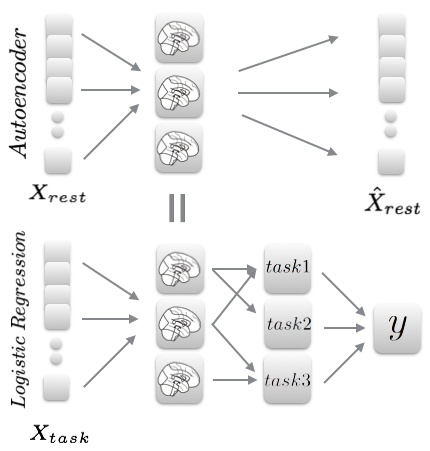
\includegraphics[width=0.40\textwidth]{figures/figure1.png}
  \vspace{-0.7cm}
  \caption {\textbf{Architecture.}
  Linear autoencoders find an optimal compression of 79,941 brain voxels
  into $n$ unknown activity patterns by improving reconstruction from them.
  The decomposition matrix equates with the bottleneck of
  a factored logistic regression.
  Supervised multi-class learning on task data ($X_{task}$)
  is thus guided by
  unsupervised decomposition of rest data ($X_{rest}$).
  }
\end{wrapfigure}
%
Autoencoders
are one-layered learning models that condense the input data to
local and global representations
by improving reconstruction from them.
%
They behave like a PCA
in case of one linear hidden layer and a squared error loss
\cite{baldi1989neural}.
This architecture yields a convex optimization objective
with unique global minimum.
Autoencoders behave like a SPCA if shrinkage terms are added to the
model weights in the optimization objective.
Moreover, they have the characteristics of an ICA in case of tied weights
and adding a nonlinear convex transformation \cite{le2011ica}.
These authors further demonstrated that ICA, sparse autoencoders, and 
sparse coding are mathematically equivalent
under mild conditions.
%
Hence, autoencoders can flexibly project the neuroimaging data
onto the main axes of variation and thus
reverse-engineer properties of the underlying
neural processes \cite{olshausen96}.

In the present investigation,
a linear autoencoder will be fed by (unlabeled) rest data and
integrated as bottleneck
into a low-rank logistic regression fed by (labeled) task data.
We can then solve the unsupervised data representation and the
supervised classification in an identical statistical learning
problem.
%
From the perspective of dictionary learning, the first layer represents
the discovered set of basis functions
whose linear combinations are learned
by the second layer \cite{olshausen96}.
%
Neurobiologically, this allows 
delineating a low-dimensional manifold of brain network patterns and then 
distinguishing mental tasks
by their most discriminative linear combinations.
%
Theoretically, a reduction in model variance should be achieved by
resting-state autoencoders that
put probability mass on the most neurobiologically
valid models in the hypothesis set.
%
Taken together,
the important modes of variation in brain dynamics and
the neural correlates subserving mental operations
have mostly been studied in isolation.
We provide a principled computational framework to link these previously
unconnected domains of systems neuroscience.

\section{Methods}
%
\paragraph{Data.}
As the currently biggest openly-accessible reference dataset,
we chose the Human Connectome Project (HCP) resources
\cite{barch2013}.
Neuroimaging task data with labels of ongoing cognitive processes
were drawn from 500 unrelated,
healthy HCP participants.
18 HCP tasks 
were selected that are known to elicit reliable neural activity
across participants.
The task paradigms include
1) working memory/cognitive control processing, 2)
incentive processing, 3) visual and somatosensory-motor processing,
4) language processing (semantic and phonological processing),
5) social cognition, 6) relational processing, and 7) emotional
processing. All data were acquired on the same Siemens Skyra 3T scanner.
Whole-brain EPI acquisitions were acquired with a
32 channel head coil (TR=720ms, TE=33.1ms, flip angle=52°, BW=2290Hz/Px,
in-plane FOV=$280\times180$mm, 72 slices, 2.0mm isotropic voxels).
The ``minimally preprocessed'' pipeline includes
gradient unwarping, motion correction, fieldmap-based EPI distortion
correction, brain-boundary-based registration of EPI to structural
T1-weighted scans, nonlinear (FNIRT) registration into MNI space,
and grand-mean intensity normalization. Activity maps were spatially
smoothed with a Gaussian kernel of 4mm (FWHM). A GLM was
implemented by FILM from the FSL suite with model regressors from convolution
with a “canonical” hemodynamic response function and from temporal derivatives.
HCP tasks were conceived to modulate activity
in a maximum of different brain regions and neural systems. Indeed, at
least 70\% of the participants showed consistent brain activity in
contrasts from the task battery, which certifies excellent
coverage \cite{barch2013}.
%
% No, this is not what is called 'coverage'
%
In sum, the HCP task data incorporated 8650 first-level activity maps
from 18 diverse paradigms administered to 498 participants (2 removed
due to incomplete data).
All maps were resampled to a common 60x72x60 space of
3mm isotropic voxels and gray-matter masked (at least 10\% tissue
probability).
The supservised analyses were based on labeled HCP task maps with
79,941 voxels of interest representing z-values in gray matter.

These labeled data were complemented by unlabeled activity maps
from HCP acquisitions of unconstrained resting-state activity.
These reflect brain activity in the absence of controlled thought.
In line with the goal of the present study, acquisition of these data was
specifically aimed at the study of task-rest correspondence.
From each participant, we included two
time-series for left and right phase encoding
with 1,200 maps of multiband, gradient-echo planar imaging acquired
during a period of 15min (TR=720 ms, TE=33.1 ms, flip angle=52°,
FOV=$280\times180$mm, and 2.0mm isotropic voxels). Besides run duration,
the task acquisitions were identical to the resting-state fMRI acquisitions
for maximal compatibility between task and rest data.
We here drew on ``minimally preprocessed'' rest data
from 200 randomly selected healthy, unrelated participants.
PCA was applied to each set of 1,200 rest maps for
denoising by keeping only the 20 main modes of
variation.
In sum, the HCP rest data concatenated
8000 unlabeled, noise-cleaned rest maps with
40 brain images from each of 200 randomly selected participants.

We were further interested in the utility of the optimal low-rank projection
in one task dataset for dimensionality reduction in another task dataset.
To this end, the HCP-derived network decompositions were used as preliminary
step in the classifcation problem of another large sample.
The ARCHI dataset \cite{pinel07} provides activity maps from
diverse experimental tasks, including auditory and visual perception, motor action,
reading, language comprehension and mental calculation.
81 right-handed healthy participants
(3 not included in present analyses due to incomplete data)
without psychiatric or
neurological history participated in four fMRI sessions acquired under
different experimental paradigms.
The functional maps were warped into
the MNI space and resampled to isotropic 3mm resolution.
Whole-brain EPI data were acquired with the same Siemens Trio with a 32
channel head coil (TR=2400ms, TE=30ms, flip angle=60°, in-plane
FOV=$19.2\times19.2$cm, 40 slices, 3.0mm isotropic voxels).
Standard preprocessing was performed with Nipype \cite{gorgo11}, including
slice timing, motion correction, alignment, and spatial normalization.
activity maps were spatially smoothed by
a Gaussian kernel of 5mm (FWHM).
Analogous to HCP data, the second task dataset incorporated 1404
labeled, grey-matter masked, and z-scored activity maps
from 18 diverse tasks acquired in 78 participants.

The labeled and unlabeled data were fed into a linear statistical model
composed of autoencoder and low-rank logistic regression.

\paragraph{Linear autoencoder.}
The affine autoencoder takes the input 
$\mathbf{x}$ and projects it into coordinates of a
latent representation $\mathbf{z}$
by

\begin{eqnarray}
  \begin{split}
    \mathbf{z} &= \mathbf{W_0} \mathbf{x} + \mathbf{b_{W_0}} \\
    \mathbf{x'} &= \mathbf{W_1} \mathbf{z} + \mathbf{b_{W_1}}
  \end{split}
  \label{eq:autoenc}
\end{eqnarray}

where $\mathbf{x \in \mathbb{R}^{d}}$ denotes the vector of $d=79,941$
voxel values from each
rest map,
$\mathbf{z \in \mathbb{R}^{n}}$ is the $n$ hidden dimensions (i.e.,
distributed neural activity patterns), and 
$\mathbf{x' \in \mathbb{R}^{d}}$
is the reconstruction vector of the original activity map
from the hidden variables. 
% XXX use bold letters for vectors and matrices
Further, $\mathbf{W_0}$ denotes the weight matrix that
transforms
from input space into the hidden space (encoder),
$\mathbf{W_1}$ is the weight matrix for back-projection
from the hidden variables to the
output space (decoder).
$\mathbf{b_{W_0}}$ and $\mathbf{b_{W_1}}$ are bias vectors.
Note that $\mathbf{W_0}$ and $\mathbf{W_1}$ are tied,
$\mathbf{W_0} = \mathbf{W_1^T}$.
The optimal model parameters $\mathbf{W_0, b_{W_0}, b_{W_1}}$ are found by
minimizing the imperfection of reconstruction according to squared error

\begin{eqnarray}
  {\mathcal{L_{AE}}}(\mathbf{x}, \mathbf{x'}) = || \mathbf{x} - \mathbf{x'} ||^2
\end{eqnarray}

This reconstruction error criterion equates with
maximizing a lower bound on the mutual information between
input and the learned representation.
Nonlinearities were not applied on the
activations in the first layer.

\paragraph{Reduced-rank logistic regression.}
Lossy compression by a low-dimensional bottleneck
is also imposed by the first layer of the low-rank
multinomial logistic regression.
It gives the probability of an input $\mathbf{x}$ to belong
to a class $i \in \mathbb{N}$

\begin{eqnarray}
  \begin{split}
    P(Y=i|\mathbf{x, V_0,V_1,b_{V_0}, b_{V_1}}) &= softmax_i(\mathbf{V_1 (V_0 x + b_{V_0}) + b_{V_1}}) \\
    &= \frac {e^{\mathbf{V_{1i} (V_{0i} x + b_{V_{0i}}) + b_{V_{1i}}}}} {\sum_j e^{\mathbf{V_{1j} (V_{0j} x + b_{V_{0j}}) + b_{V_{1j}}}}}            
  \end{split}
  \label{eq:lr}
\end{eqnarray}

where the matrix $\mathbf{V_0 \in \mathbb{R}^{dxn}}$
transforms the input $\mathbf{x \in \mathbb{R}^{d}}$
into $n$ latent components
and the matrix $\mathbf{V_1 \in \mathbb{R}^{nxc}}$
projects the latent components
onto hyperplanes that reflect $c$ class probabilities.
$\mathbf{b_{V_0}}$ and $\mathbf{b_{V_1}}$ are corresponding
bias vectors.
The loss function is given by

\begin{eqnarray}
  \begin{split}
    {\mathcal{L_{LR}}}(\mathbf{x, y}) = \frac{1}{N_{X_{task}}} \sum_{i=0}^{N_{X_{task}}} \log(P(Y=y^{(i)}|\mathbf{x^{(i)}; V_1 (V_0 x + b_{V_0}) + b_{V_1}})
\end{split}
\label{eq:lr_loss}
\end{eqnarray}

\paragraph{Layer combination.}
Importantly, the optimization problem of the linear autoencoder
and the low-rank logistic regression
are linked one two levels. First, their transformation matrices mapping from
input to the latent space are identical
\begin{eqnarray}
  \mathbf{V_0} = \mathbf{W_0}
\end{eqnarray}
We thus search for a compression of the 79,941 voxel values into $n$ latent
components that represent an optimal latent code for both
rest and task activity data.
Second, the objectives of the autoencoder and the low-rank
logistic regression are interpolated in the common loss function

\begin{eqnarray}
  \begin{split}
{arg\,min}_\theta \hspace{0.2cm} {\mathcal{L}}(\theta, \lambda) = \lambda {\mathcal{L_{LR}}}
+ (1-\lambda)\frac{1}{N_{X_{rest}}} {\mathcal{L_{AE}}} + \ell_1(\theta) + \ell_2(\theta)
  \label{eq:loss_equ}
\end{split}
\end{eqnarray}

In so doing, we search for the combined model parameters
$\theta=\{\mathbf{V_0,V_1,b_{V_0}, b_{V_1}, b_{W_0}, b_{W_1}}\}$
with respect to the (unsupervised) reconstruction error and the
(supervised) task classification.
${\mathcal{L_{AE}}}$ is devided by ${N_{X_{rest}}}$ to equilibrate both
loss terms to the same order of magnitude.
For parameter shrinkage, we
impose a combination of $\ell_1$ and $\ell_2$ penalties
$\forall p \in \theta$ (i.e., elasticnet).

\paragraph{Optimization.}
The common objective was approximated 
% XXX why 'approximated' ?
in the neuroimaging data
by updating parameters by derivates 
% XXX derivates ???
of the 
semi-supervised low-rank logistic regression.
The required gradients are easily obtained by using the chain rule to
backpropagate error derivatives through the linear network.
As solver, we chose \textit{rmsprop} \cite{rmsprop},
a mini-batch version of rprop.
This procedure dictates an adaptive learning rate
for each model parameter by
scaled gradients from a running average.
Gradient normalization by rmsprop
is known to effectively exploit curvature information.
We opted for a small batch size of $100$, given the high degree of
redundancy in $X_{rest}$ and $X_{task}$.
The matrix parameters were initalized by Gaussian random values multiplied
by a gain of $0.004$. The bias parameters were initalized to zero.
With a slight abuse of notation, let $\theta$ denote a component of $\theta$.
The normalization factor and the update rule for $\theta$
are given by

\begin{eqnarray}
  \begin{split}
    \mathbf{v^{(t+1)}} &= \rho \mathbf{v^{(t+1)}} + (1 - \rho)\left(\frac{\partial f}{\partial \theta}\right)^2
%v^{(t+1)} = \rho v^{(t+1)} + (1 - \rho)˜|\nabla f
\\
\theta^{(t+1)} &= \theta^{(t)} + \alpha \frac{\nabla f(\theta^{(t)})}{\sqrt{\mathbf{v^{(t+1)}} + \epsilon}},
  \end{split}
\end{eqnarray}

where $0 < \rho < 1$ constitutes the decay rate. $\rho$ was set to
$0.9$ to deemphasize the magnitude of the gradient.
Further, $\alpha$ is the learning rate and $\epsilon$ a global damping factor.
The hyper-parameter $\alpha$ was set to $0.00001$ by prior studies and $\epsilon$ was set to $10^{-6}$.
%
Note that we have also experimented with other solvers
(stochastic gradient descent, adadelta, and adagrad) but found that
rmsprop converged faster and with higher generalization performance.

\paragraph{Hints.}
In fact, the constraint by a rest-data autoencoder qualifies as a
\textit{hint}
rather than regularization in a strict sense \cite{abu1994hints}.
Its purpose is not to prevent overfitting but to introduce
prior knowledge on known properties of the unknown target function $f$.
Rather than only relying on input-output pairs in the learning process,
we thus narrow our hypothesis set to the biologically most plausible solutions.
That is, we reduce the search space in a way that
is compatible with the expected representation of BOLD activity signals.

\paragraph{Implementation.}
The analyses were performed in Python.
We used \textit{nilearn} to handle
the high-dimensional neuroimaging data 
\cite{abrah14}
and
\textit{theano} for automatic, numerically stable
differentiation of symbolic computation graphs
\cite{bastien2012theano, bergstra2010theano}.
All Python scripts that generated the results are
accessible online for reproducibility and reuse
\url{http://github.com/anonymous/anonymous}.
% url{http://github.com/banilo/nips2015}.

\bigskip
\begin{figure}
\begin{centering}
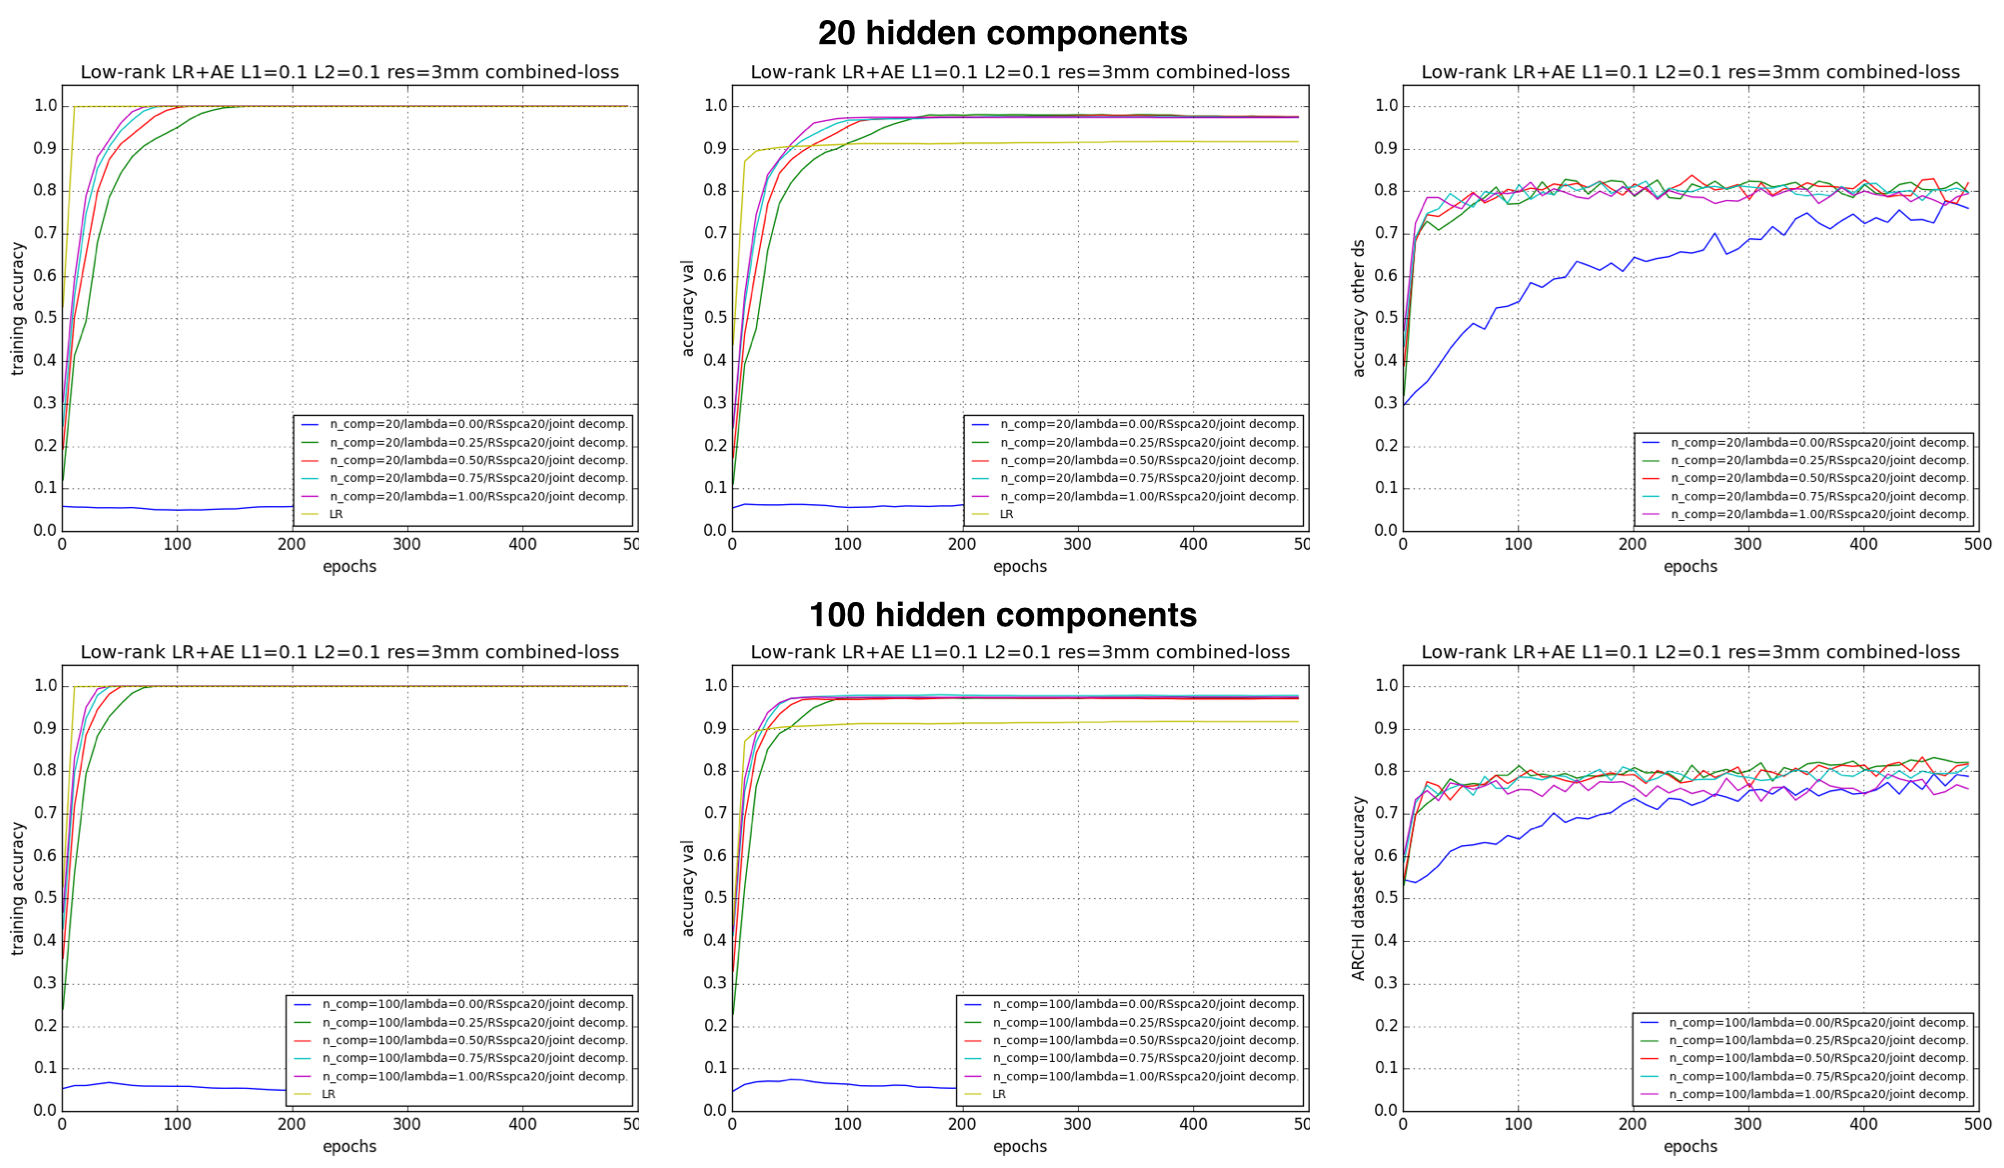
\includegraphics[width=1.00\textwidth]{figures/accuracies.png}
\end{centering}
\caption{\textbf{Generalization performance}
Depicts in-sample (apply current model on training set, \textit{left column}),
out-of-sample (current model on test set, \textit{middle column}),
and out-of-dataset (compress other dataset using the
learned decomposition for classification, \textit{right column}) accuracy.
Curves for different choices of $\lambda$ as well as for ordinary
logistic regression (\textit{yellowish})
across iterations over the HCP task data (epochs).
XXX: Message ??
}
\end{figure}

\begin{figure}
\begin{centering}
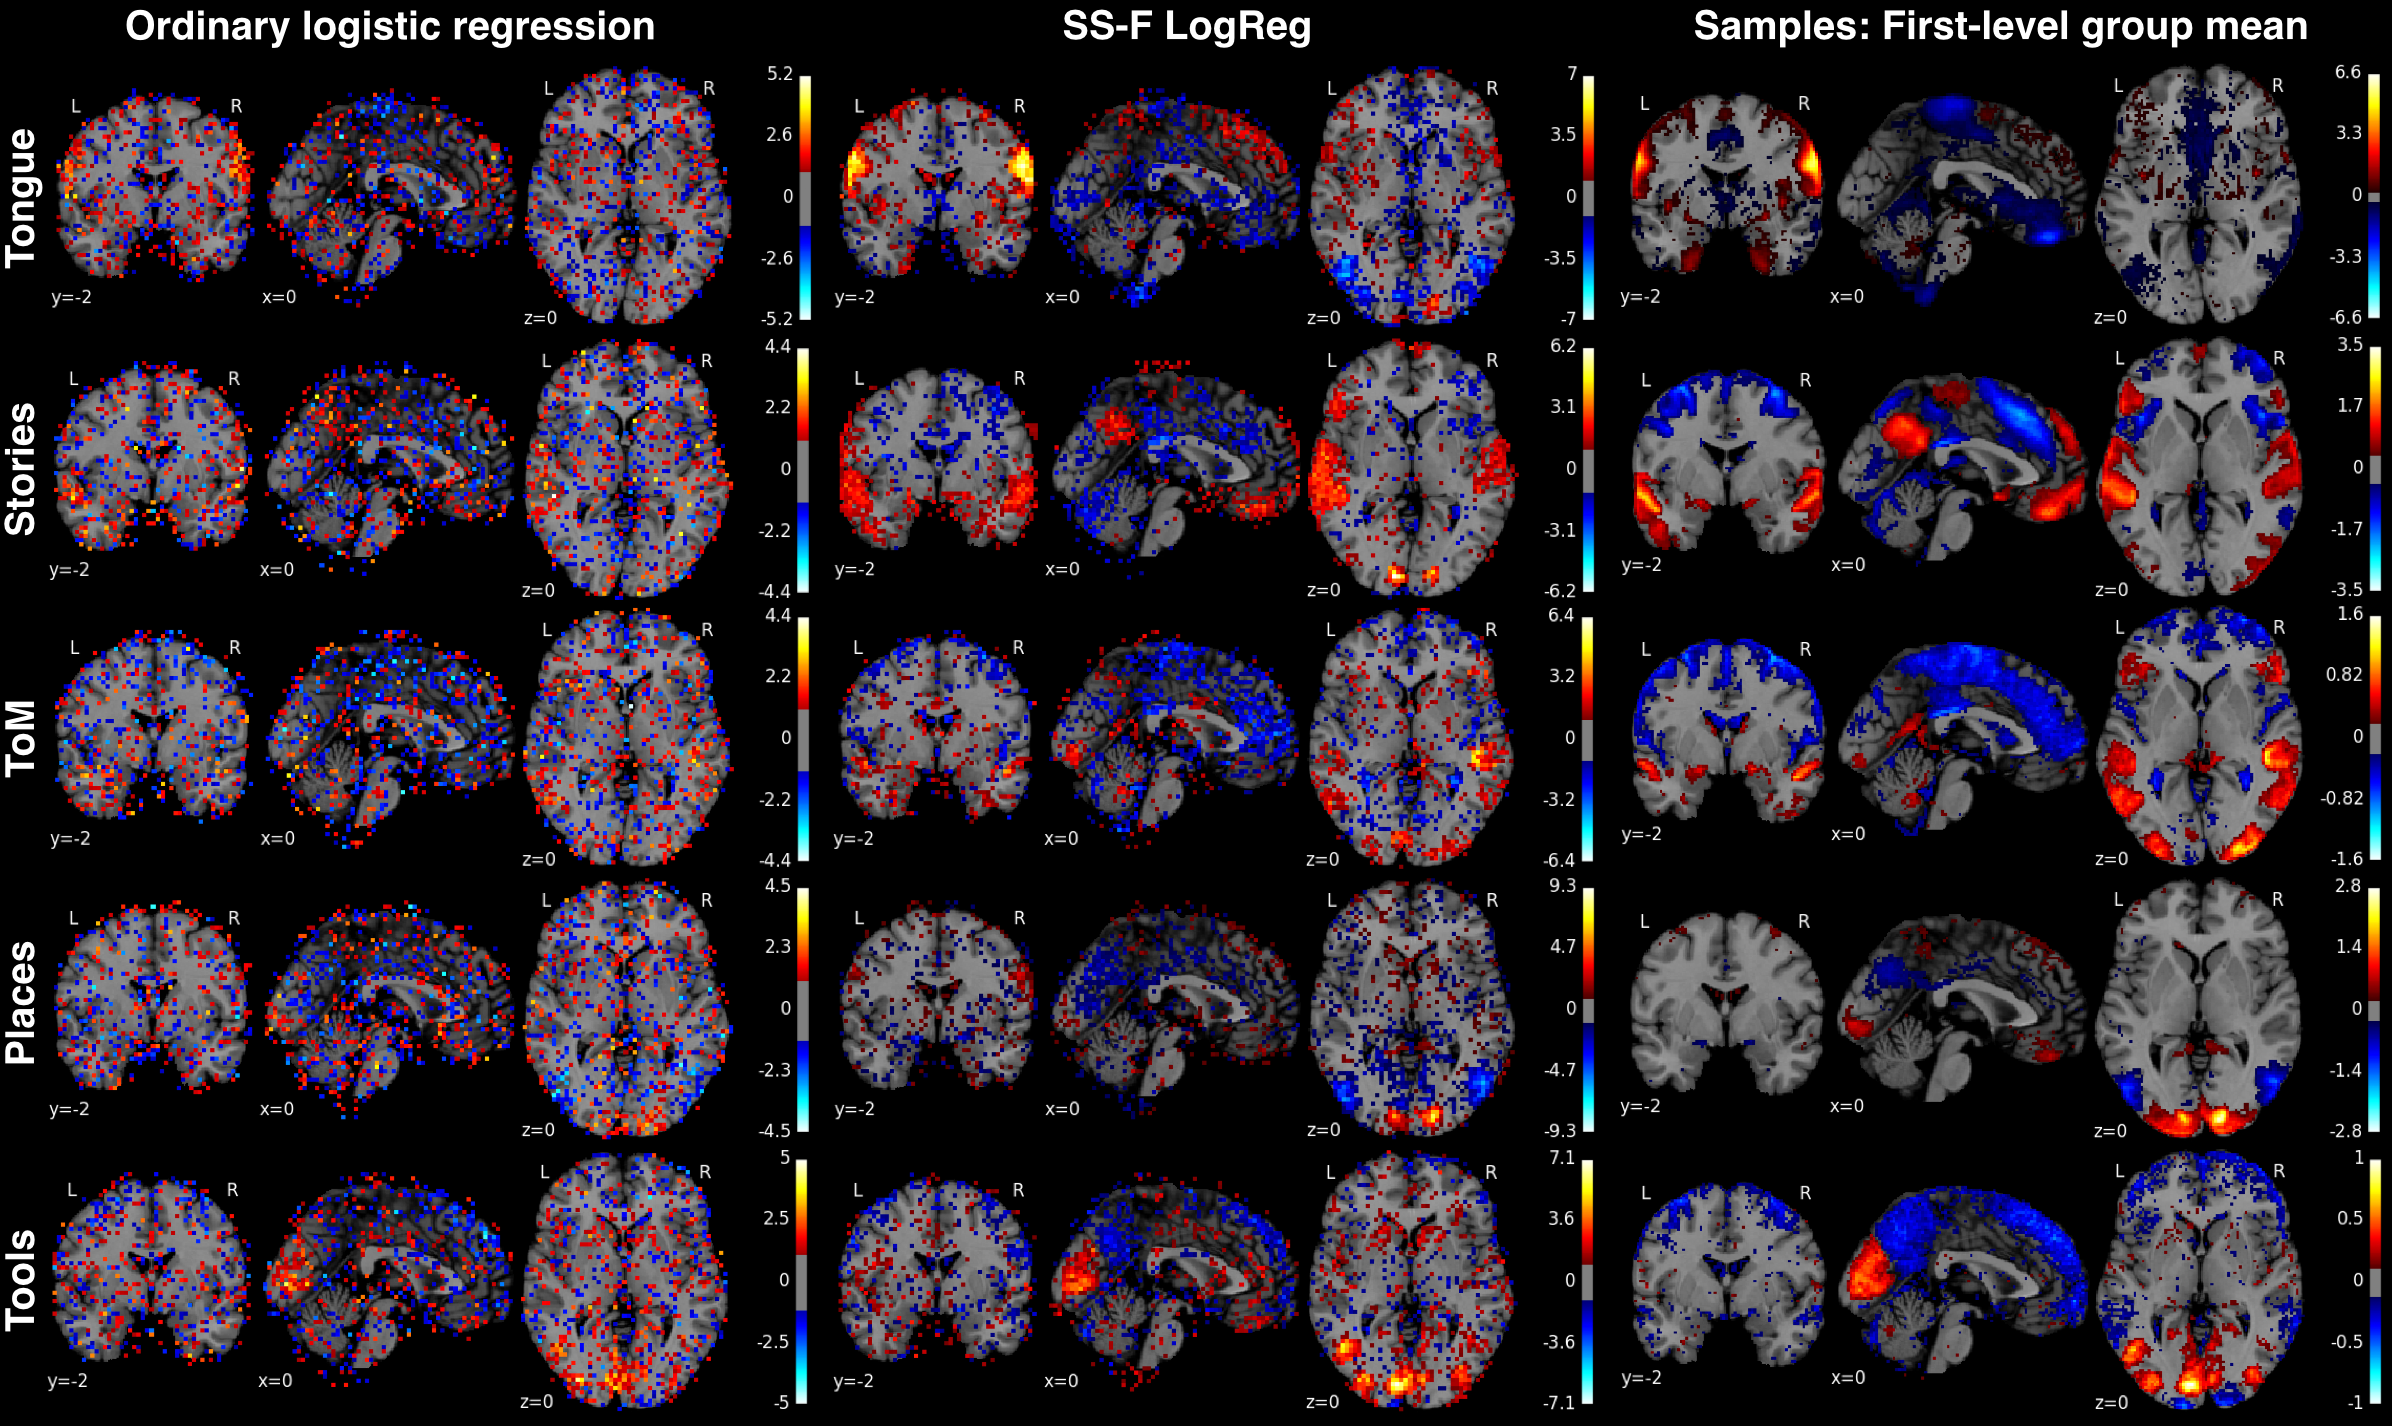
\includegraphics[width=1.00\textwidth]{figures/figure_weights_perc75.png}
\end{centering}
\caption{\textbf{Interpretability of classification weights}
The voxel predictors corresponding to 5 exemplary
(of 18 total) psychological tasks (\textit{rows})
from the HCP dataset \cite{barch2013}.
\textit{Left column:} ordinary logistic regression (same
implementation but without bottleneck or autoencoder),
\textit{middle column:} semi-supervised low-rank logistic regression
($n=20$ latent components, $\lambda=0.5$, $\ell_1=0.1$, $\ell_2=0.1$),
\textit{right column:} voxel-wise average of whole-brain
activity maps from each task.
Low-rank logistic regression
a) puts higher absolute weights on relevant structure
b) lower ones on irrelevant structure,
and
c) yields BOLD-typical local contiguity.
All values are z-scored and thresholded at the 75th percentile.
}
\end{figure}

\begin{figure}
% XXX: figure not readable
\begin{centering}
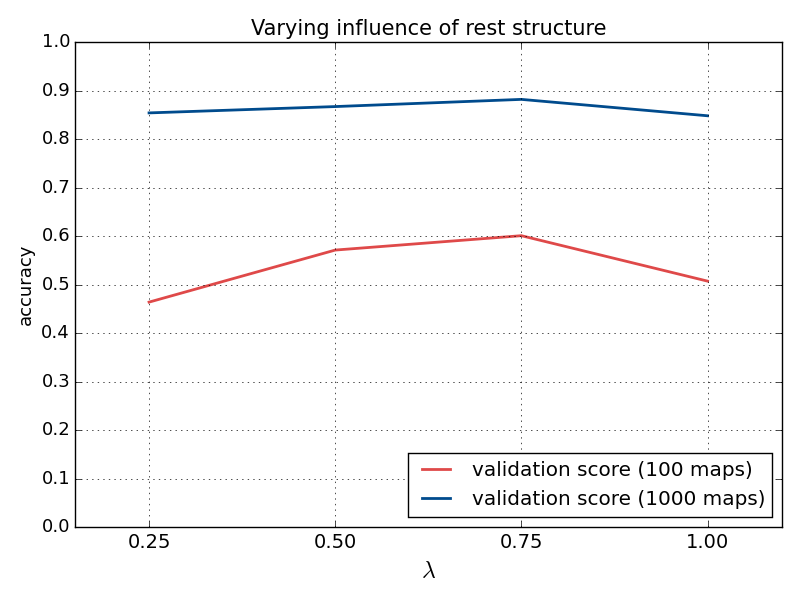
\includegraphics[width=1.00\textwidth]{figures/semisup.png}
\end{centering}
\caption{\textbf{Relation between support recovery and out-of-dataset performance}
\textit{Upper row:} the fit-for-purpose of the classification models
is quantified by linear correlation between the
z-scored average task image and the z-scored weights from
ordinary (\textit{red}) and present (\textit{blue colors}) logistic
regression ($\lambda=0.25, 0.50, 0.75, 1.00$).
\textit{Lower row:} ordinary logistic regression is applied to the
ARCHI dataset after projection into the latent dimensions learned from
the HCP task data.

\textbf{whenever I tried to have 3+ times more rest than task images results dropped dramatically...naive interpretation: if the rest information is too rich it overrules task patterns and hinders the supervised learning
}
}
\end{figure}

\section{Experimental Results}
\paragraph{Serial versus parallel structure discovery and classification.}
We first tested for an advantage of combined unsupervised decomposition
and supervised classification learning.
We benchmarked against
performing data reduction on the (unlabeled)
first half of the HCP data by ICA and SPCA ($n=5, 20, 50, 100$ components)
and learning classification models in the (labeled) second half
by ordinary logistic regression.
%
ICA performed iterative blind source separation
by a parallel FASTICA implementation (200 maximum iterations,
per-iteration tolerance of 0.0001,
initialized by random mixing matrix, whitening).
SPCA separated the BOLD signals into
network components with few regions by
a regression-type optimization problem constrained by
$\ell_1$-penalty
(no orthogonality assumptions, 1000 maximum iterations,
per-iteration tolerance of 1 * 10\textsuperscript{-8}, sparsity
alpha=1).
%
The second half of the data was projected onto the
latent components discovered in first data half.
The ensuing component loadings were submitted to ordinary
logistic regression
(one hidden layer, $\ell_1=0.1$, $\ell_2=0.1$, 500 maximum iterations).
%
This 2-step approaches were compared against semi-supervised low-rank
logistic regression
(SS-LR LogReg, two hidden layers, $\ell_1=0.1$, $\ell_2=0.1$,
500 maximum iterations, $\lambda=0.75$).
Importantly, all trained classification models were tested
on a large, unseen test set (20\% of data) in the presented analyses.
%
Across choices for $n$, SS-LR LogReg
achieved more than 96\% out-of-sample accuracy, whereas
supervised learning based on ICA and SPCA loadings
ranged from 37,53\% to 87,28\%
and
32,19\% to 83,97\%, respectively (Table \ref{table_one}).
%
These explorations attest to the advantage of directly searching for
classification-relevant structure in the fMRI data,
rather than solving supervised and unsupervised problems independently.
This effect was particularly pronounced when assuming few hidden dimensions.

\begin{table}[h]
 \centering
 \resizebox{0.4\textwidth}{!}{%
 \begin{tabular}{lccc}
 \hline
 \textit{n}               & ICA + LogReg & SPCA + LogReg & SS-LR LogReg \\ \hline
 \multicolumn{1}{l|}{5}   & 37,53 \%     & 32,19 \%      & 96,50 \%     \\
 \multicolumn{1}{l|}{20}  & 80,98 \%     & 78,15 \%      & 97,33 \%     \\
 \multicolumn{1}{l|}{50}  & 84,19 \%     & 83,97 \%      & 97,69 \%     \\
 \multicolumn{1}{l|}{100} & 87,28 \%     & 82,19 \%      & 97,80 \%     \\ \hline
 \end{tabular}
 }
 \vspace{-0.2cm}
 \caption{Serial versus parallel dimensionality reduction and classification}
 \label{table_one}
 \end{table}

\paragraph{Model performance.}
\begin{itemize}
\item{20 components: high bias/low variance
100 compoentens: low bias/high variance}
\end{itemize}
\begin{itemize}
  \item{This was evaluated by the prediction
accuracy on a validation set (20\% of the training data) at each iteration
over the ARCHI task data}
  \item{the less lambda, the faster the convergence, with small differences
  though; smaller differences with larger number of components}
  \item{both 20 and 100 hidden components achieve 97\% out-of-sample
  accuracy}
  \item{ordinary logistic regression converges faster but with stagnation at
  92\% out-of-sample accuracy}
  \item{classification at chance 6\% in case of lambda==0 because 
  only the unsupervised layer of the estimator is optimized}
  \item{important: the thus only resting-state-trained decomposition achieves
  the same usefulness in the ARCHI classification than the
  decomposition derived in semi-supervised fashion}

out of sample performance: extract features of general relevance
beyond the supervised problem at hand
\end{itemize}

\begin{table}[h]
  \centering
  \resizebox{1.00\textwidth}{!}{%
\begin{tabular}{l|cccc|llllcccc|llll|}
  \hline
                            & \multicolumn{4}{c|}{\textit{n = 5}}                                                                                                                & \multicolumn{4}{c|}{\textit{n = 20}}                                                                                                                       & \multicolumn{4}{c}{\textit{n = 100}}                                                       \\ \hline
  \textit{}                 & \multicolumn{1}{l}{$\lambda=0.25$} & \multicolumn{1}{l}{$\lambda=0.50$} & \multicolumn{1}{l}{$\lambda=0.75$} & \multicolumn{1}{l|}{$\lambda=1.00$} & \multicolumn{1}{l}{$\lambda=0.25$}   & \multicolumn{1}{l}{$\lambda=0.50$}   & \multicolumn{1}{l}{$\lambda=0.75$}   & \multicolumn{1}{l|}{$\lambda=1.00$}   & $\lambda=0.25$   & $\lambda=0.50$   & $\lambda=0.75$   & \multicolumn{1}{l}{$\lambda=1.00$} \\ \hline
  Out-of-sample\\accuracy   & \textit{88,90\%}                   & 95,13\%                            & \textbf{96,49\%}                   & 95,72\%                             & 97,44\%                              & \textbf{97,80\%}                     & 97,33\%                              & \textit{97,32\%}                      & 97,21\%          & \textit{97,03\%} & \textbf{97,80\%} & 97,38\%                            \\
  Precision (mean)          & \textit{86,98\%}                   & 94,86\%                            & \textbf{96,28\%}                   & 95,36\%                             & \textbf{97,38\%}                     & 97,06\%                              & \textit{96,98\%}                     & 97,02\%                               & 96,90\%          & \textit{96,47\%} & \textbf{97,50\%} & 96,91\%                            \\
  Recall (mean)             & \textit{88,27\%}                   & 95,19\%                            & \textbf{96,57\%}                   & 95,70\%                             & \textbf{97,51\%}                     & 97,50\%                              & \textit{97,35\%}                     & 97,36\%                               & 97,20\%          & \textit{97,15\%} & \textbf{97,88\%} & 97,37\%                            \\
  F1 score (mean)           & \textit{86,64\%}                   & 94,89\%                            & \textbf{96,38\%}                   & 95,43\%                             & \textbf{97,42\%}                     & 97,22\%                              & \textit{97,11\%}                     & 97,13\%                               & 97,00\%          & \textit{96,71\%} & \textbf{97,65\%} & 97,07\%                            \\ \hline
  Out-of-dataset \\accuracy & 60,83\%                            & \textit{54,30\%}                   & 60,69\%                            & \textbf{62,92\%}                    & 79,72\%                              & \textbf{81,94\%} & 79,72\%           & \textit{79,44\%}                     & \textbf{82,08\%} & 81,66\%            & 81,25\%          & \textit{75,83\%}                   \\ \hline
  \end{tabular}

}
\end{table}

\paragraph{Feature identification.}
\begin{itemize}
  \item{fit for purpose; the right model should have
  high probability in the right places}
  \item{comparing to ordinary logistic regression, low-rank logreg yielded class weights 
  that were much more similar to feature of the respective training examples,
  for any choice of $\lambda$}
  \item{the higher $\lambda$, the better support recovery}
  \item{conversely, the higher lambda (i.e., bigger emphasis on the
  resting-state autoencoder), the more useful the low-dimensional transformations
  for classification in an independent dataset (ARCHI) as measured by f1 score
  for higher (i.e., 50 and 100) but not lower (i.e., 20) numbers
  of latent components}

support recovery:
Low-rank logistic regression
a) puts higher absolute weights on relevant structure
b) lower ones on irrelevant structure,
and
c) yields BOLD-typical local contiguity.

the features of the classes show that we captured activaiton properties,
not particpant or paradigm properties
\end{itemize}

\paragraph{Miscellaneous observations.}
For the sake of completeness,
we informally report modifications of the model
that did not improve the generalization performance.
%
Introducing stochasticity into model learning by 
a) input corruption of $\mathbf{X_{task}}$ or
b) drop-out at the bottleneck $\mathbf{W_0}$ using binomial
distributions ($p=0.1, 0.3, 0.5$) deteriorated model performance
in all instances. 
%
Adding c) rectified linear units (ReLU) to $\mathbf{W_0}$ or
other commonly used nonlinearities (d) sigmoid, e) softplus,
f) hyperbolic tangent) all led to smaller classification accuracies.
%
Further, g) ``pretraining'' of the bottleneck $\mathbf{W_0}$
(i.e., non-random initialization) by 
either corresponding SPCA or ICA loadings did not exhibit improved accuracies,
neither did h) autoencoder pretraining.
%
Moreover,
introducing an additional i) overcomplete layer (100 units)
after the bottleneck was not advantageous.
%
Finally, imposing imposing either j) only $\ell_1$-penalty or 
k) only $\ell_2$-penalty was disadvantageous in all tested cases,
which favored elasticnet regularization chosen in the above analyses.

\section{Discussion and Conclusion}
% Conceptual recap+gain of current paper
Using the flexibility of autoencoders, we
learn the optimal decomposition from high-dimensional
voxel brain space into the most important activity patterns for a
supervised learning question.
The higher generalization accuracy and support recovery, comparing to
ordinary logistic regression, hold potential
for adoption in various neuroimaging analyses.
Besides increased performance, these models are more interpretable by
automatically learning a mapping to and from a brain-network space.
This domain-specifc classification algorithms
encourages departure from the artificial and statistically
less attractive voxel space.
Neurobiologically,
neural activity underlying defined mental operations
can be explained by linear combinations of the main activity
patterns. That is,
fMRI data probably concentrate near
a low-dimensional manifold of brain networks.
Extracting fundamental building blocks of brain organization might
facilitate the quest for the cognitive primitives of
human thought.
We hope that these first steps stimulate development towards
powerful semi-supervised classification methods in systems neuroscience.

% grand perspective
In the future, automatic reduction of brain images to
their neurobiological essence
may leverage data-intense neuroimaging studies.
Initiatives for data collection are rapidly increasing
in neuroscience \cite{poldrack2014data}.
These promise structured integration
of accumulating neuroscientific knowledge from neuroimaging databases.
Tractability by
condensed feature representations can avoid the ill-posed problem of
learning the full distribution of activity patterns.
%
This is not only relevant to the 
multi-class challenges spanning the human cognitive space
\cite{schwartz2013mapping}
but also the
multi-modal combination with
high-resolution 3D models of brain anatomy \cite{amunts2013bigbrain}
and
high-throughput genome analyses \cite{need2010gwas}.
%
The biggest socioeconomic potential may
lie in across-hospital clinical studies that
predict disease trajectories and drug responses
in psychiatric/neurological populations
\cite{frackowiak2015future, gustav2011cost}.

\paragraph{Acknowledgment}
{\small
Data were provided by the Human Connectome Project. The study was supported
by the German National Academic Foundation (D.B.).
}

\small
\bibliographystyle{splncs03}
\bibliography{nips_refs}

\end{document}
